\chapter{Published Work}
\label{chapter:publishedWorks}
\index{Published work}

We have published several research studies based on the application to multi-objective metaheuristics to solve the molecular docking problem. Specifically, four articles have been published in journals indexed in the Journal of Citation Report (JCR) from the Institute of Scientific Information. In addition to this, four articles have been published in congresses. Two of them have been published in international congresses and the rest in national congresses.

\section{List with Research Contributions}

These four JCR articles apply metaheuristics to solve the molecular docking problem. These contributions can be organized as follows:\\

\noindent \textbf{Articles published in journal indexed in JCR:}

\begin{itemize}[leftmargin=5.5mm]
	
	\item \fullcite{lopez14jmetalcpp}\\Impact Factor: 4,981. Q1 (3/57)  in the category of mathematical and computational biology.
	
	\item \fullcite{lopez2015asoc}\\Impact Factor: 2,857. Q1 (21/130) in the category of Computer Science and Artificial Intelligence.
	
	\item \fullcite{Molecules2015}\\Impact Factor: 2,465. Q2 (25/59) in the category of Chemistry, Organic.
	
	\item \fullcite{Molecules2016}\\Impact Factor: 2,465. Q2 (25/59) in the category of Chemistry, Organic.
	
\end{itemize}

\noindent \textbf{Articles published in international congresses:}

\begin{itemize}[leftmargin=5.5mm]
	
	\item \fullcite{LopezCamacho2016AlCoB}
	
	\item \fullcite{GarciaNieto2016ANTS}

\end{itemize}

\noindent \textbf{Articles published in national congresses:}

\begin{itemize}[leftmargin=5.5mm]
	
	\item \fullcite{lopez2015maeb}
	
	\item \fullcite{lopez2016maeb}  

\end{itemize}

\section{Summary of the articles that support the thesis}
\label{sec:Summary_articles_support}

This section summarizes the articles that support this thesis. All these papers are related to the application of the single-objective and multi-objective optimizations to solve the problem of the molecular docking. In the first article, we have described the integration of AutoDock and jMetal and its application in the domain of molecular docking. In the second published article, we have performed a study comparing the mono-objective techniques using a set of flexible instances. In a third and fourth study, we have applied a set of multi-objective metaheuristics that optimize two objectives, guiding the algorithm to search the best molecular docking solutions.

\subsection{jMetalCpp: optimizing molecular docking problems with a C++ metaheuristic framework}

\textbf{Reference:}~\cite{lopez14jmetalcpp} \fullcite{lopez14jmetalcpp}\\
Pages in this thesis: \pageref{start-pdf/bioinformatics.pdf}-\pageref{stop-pdf/bioinformatics.pdf}

In~\cite{lopez14jmetalcpp} we introduced jMetalCpp, the C++ version of the metaheuristic framework jMetal (originally written in Java). We also presented the combination of this software with the widely used AutoDock, which is the most used tool to solve molecular docking problems. The inclusion of jMetalCpp inside the AutoDock provided the latter several additional metaheuristic techniques to solve molecular docking problems. Both new softwares (the standalone jMetalCpp and the ``fusion'' of jMetalCpp with AutoDock) were published online\footnote{http://jmetalcpp.sourceforge.net/}$^{,}$\footnote{http://khaos.uma.es/autodockjmetal/} to be freely used by the scientific community.

\subsection{Solving molecular flexible docking problems with metaheuristics: a comparative study}

\textbf{Reference:}~\cite{lopez2015asoc} \fullcite{lopez2015asoc}\\
Pages in this thesis: \pageref{start-pdf/asoc.pdf} -- \pageref{stop-pdf/asoc.pdf}

In our first single-objective study~\cite{lopez2015asoc}, we tested the performance of new metaheuristic techniques apart from those included in the AutoDock Tools for solving molecular docking problems. This study approached the problem as a single-objective optimization problem, as AutoDock does. AutoDock provides two different techniques to solve the problem: a Lamarckian Genetic Algorithm (LGA), which includes local search, and a common Genetic Algorithm (GA). We added four single-objective metaheuristic: generational Genetic Algorithm (gGA), steady-state Genetic Algorithm (ssGA), Differential Evolution (DE) and Particle Swarm Optimization (PSO). A study with 75 protein-ligan complexes taken from PDB was carried on using the same fitness function and configuration parameters than AutoDock to have a comparison as fair as possible. The objective was the binding energies in kcal/mol associated with the receptor-ligand complex, as explained in Section~\ref{subsection:mono_solution}. Therefore, the lower the binding energy the better the result.

This study had two different steps. In the first one, we tuned the parameter configuration of the four single-objective metaheuristic techniques. In order to do so, we selected 11 protein-ligand complexes taken from the PDB database. After we obtained a set of configuration parameters for the 4 single-objective metaheuristics, a thorough comparison was made between these four and the algorithms provided by AutoDock. This time, a set of 75 instances also from PDB were used.

It was demonstrated that DE (jMetal) obtained the best results in 67 of the 75 instances, followed by LGA (AutoDock) that achieved the best results in the remaining eight instances (1B6L, 1BDL, 1HEF, 1HIV, 1HPO, 1K6C, 1Z1H and 1ZIR). These results were provided with statistical confidence ($\alpha = 0.05$) as a series of non-parametric statistical tests were applied. In particular, Friedman's ranking and Holm's post-hoc multicompare tests were calculated and showed that DE achieved a statistically better performance than the rest of the other analyzed algorithms. This fact is remarkable as the AutoDock algorithms are specifically designed to solve molecular docking problems.
It was also noted that DE showed a slower convergence behavior, though with more successful solutions than its competitors. However, gGA demonstrated a fast convergence, and also achieved high-quality solutions, so this algorithm could be a good choice when looking for fast, but good enough solutions.

\subsection{A new multi-objective approach for molecular docking based on RMSD and binding energy}

\textbf{Reference:}~\cite{LopezCamacho2016AlCoB} \fullcite{LopezCamacho2016AlCoB}\\
Pages in this thesis: \pageref{start-pdf/alcob.pdf} -- \pageref{stop-pdf/alcob.pdf}

This work was presented in the 3rd International Conference on Algorithms for Computational Biology (AlCoB 2016), celebrated in Trujillo, Spain in June of 2016. It was derived from the idea of taking a multi-objective optimization approach to solve molecular docking problems. In the beginning, the strategy we had followed was to decompose the final binding energy (the minimization objective of the previous work) into several components, particularly the intra- and inter-molecular energy~\cite{Molecules2015}. After that, it was decided to use as objectives the same energy taken in the single-objective study and the RMSD. These concepts were explained in more detail in Section~\ref{subsection:multi_solution}.

However, in this paper~\cite{LopezCamacho2016AlCoB}, we selected four representative multi-objective optimization algorithms such as NSGA-II, GDE3, SMPSO and MOEA/D. A benchmark composed of 11 complexes having receptor and ligand flexibility was selected. The selection of these complexes was motivated as they are docking problems containing a wide range of ligand sizes (from small to large inhibitors). Two quality indicators were calculated to measure the performance of each algorithm: Hypervolume (I$_{HV}$) and Unary Additive Epsilon Indicator ($I_{\epsilon+}$). The first indicator takes into account both convergence and diversity, whereas the second one ($I_{\epsilon+}$) gives a measure of the convergence degree of the obtained Pareto front approximations. It is worth noting that, as we are dealing with real-world optimization problems, the true Pareto fronts needed to calculate these metrics are not known, so they had to be obtained using all the approximated fronts from all the executions of all the multi-objective algorithms for each problem.

The $I_{HV}$ is the sum of the contributed volume of each point of a front in respect to a reference point, so the higher the convergence and diversity degrees of a front, the higher its $I_{HV}$ value. According to these results, SMPSO achieved the best $I_{HV}$ values in all the eleven problems, being MOEA/D the second best performing technique. It is important to note that many algorithms had a $I_{HV}$ value equal to zero, this happens when all the points of the produced fronts are beyond the limits of the reference point. This happened in most of the problems in all the algorithms excepting SMPSO, what leaded us to think that we are facing a hard optimization problem.
Also, SMPSO achieved the best performance results according the $I_{\epsilon+}$ indicator (in this case, the lower the value, the better). SMPSO achieved the best values for all 11 instances except for 1HTF, in which it got the second best value. MOEA/D, which was the algorithm that got the best value for 1HTF, achieved the second best values for 9 instances. GDE3 got the second best value in one instance (1HPX) while NSGA-II got the worst results for all the instances.

After this work was presented, it was invited to be substantially extended and be submitted to a special issue of the journal IEEE/ACM Transactions on Computational Biology and Bioinformatics (TCBB, 2014 JCR impact factor: 1.438, quartile Q1). To this day, it is still under-review.

\subsection{A study of archiving strategies in multi-objective PSO for molecular docking}

\textbf{Reference:}~\cite{GarciaNieto2016ANTS} \fullcite{GarciaNieto2016ANTS}\\
Pages in this thesis: \pageref{start-pdf/ants.pdf} -- \pageref{stop-pdf/ants.pdf}

This work~\cite{GarciaNieto2016ANTS} was presented in the 10th International Conference on Swarm Intelligence (ANTS 2016), celebrated in Brussels, Belgium in September of 2016. It is the natural continuation from the previous one, where we obtained that SMPSO obtained best overall results when applying a multi-objective approach to solve molecular docking problems. The previous experiment was replicated using several SMPSO variants based on different archiving strategies. The selected variants are: SMPSO$_{hv}$, SMPSOD and SMPSOC. The original SMPSO and OMOPSO (the algorithm which SMPSO was inspired from) were also included in the comparison.

This paper introduced the variant named SMPSOC. It is characterized by the use of a cosine similarity when calculating the density value of each point in the solution front. The variant SMPSOD was also presented in this paper for the first time. It is an archive-less approach, implemented as an aggregative version of SMPSO inspired by MOEA/D.

According to the $I_{HV}$ indicator, SMPSO$_{hv}$ obtained the best results for all the 11 instances, whereas SMPSOD got the second best value in 6 instances, SMPSOC in three and the original SMPSO in two, respectively. In the same manner, SMPSO$_{hv}$ obtained again the best values for the 11 instances according to the $I_{\epsilon+}$ indicator. The second best values were achieved by SMPSOD in 7 instances, the original SMPSO in three and SMPSOC in one instance, respectively.

\section{Summary of other publications related to this thesis}

This section briefly comments the other four articles that do not support this thesis but are related to its topic. Two of them were published in the Molecules journal and the other two were published in national congresses.

In \cite{Molecules2015}, we presented our first multi-objective approach. The final binding energy (the minimization objective of the mono-objective study) was decomposed into the intra- and inter-molecular energy. These two components were used as two contrary objectives. We selected six multi-objective optimization algorithms such as NSGA-II, ssNSGA-II, GDE3, SMPSO, MOEA/D and SMS-EMOA. A heterogeneous set of 11 protein-ligand complexes with flexible ligands and receptors was selected in order to carry out the experiments. A use case of drug discovery that involves the aeroplysinin-1 compound and the human Epidermal Growth Factor (EGFR) was also provided. The results demonstrated that according to the use casses presented, it can be more interesting to select a specific docking solution with a balanced tradeoff between the E$_{inter}$ and E$_{intra}$ values.

In \cite{Molecules2016}, we presented our latest multiobjective approach. This time, we selected the final binding energy and the RMSD as optimization objectives and NSGA-II, GDE3, SMPSO and MOEA/D as multi-objective optimization algorithms. In this study, we performed an analysis on binding sites in the EGFR kinase domain and molecular interactions. The use cases were based on instances with wild-type EGFR, EGFR with mutations L858R and G719S and EGFR double mutants (T790M/L858R and T790M/G719S). This proposed approach can be used for in silico studies to test other analog kinase inhibitors or similar compounds for drug discovery in those cancers in which therapeutic targets are changed by somatic mutations.

The two latter articles where published in the X and XI `Congreso Español de Metaheurísticas, Algoritmos Evolutivos y Bioinspirados (MAEB)' in 2015 and 2016. The first article \cite{lopez2015maeb} presented our first multi-objective approach (using the intra- and inter-molecular energy as contrary objectives). The following year, we presented our multi-objective PSO study in this same congress \cite{lopez2016maeb}.

\section{Copies of the articles that support the thesis}

This section includes copies of the four articles summarized in Section \ref{sec:Summary_articles_support}

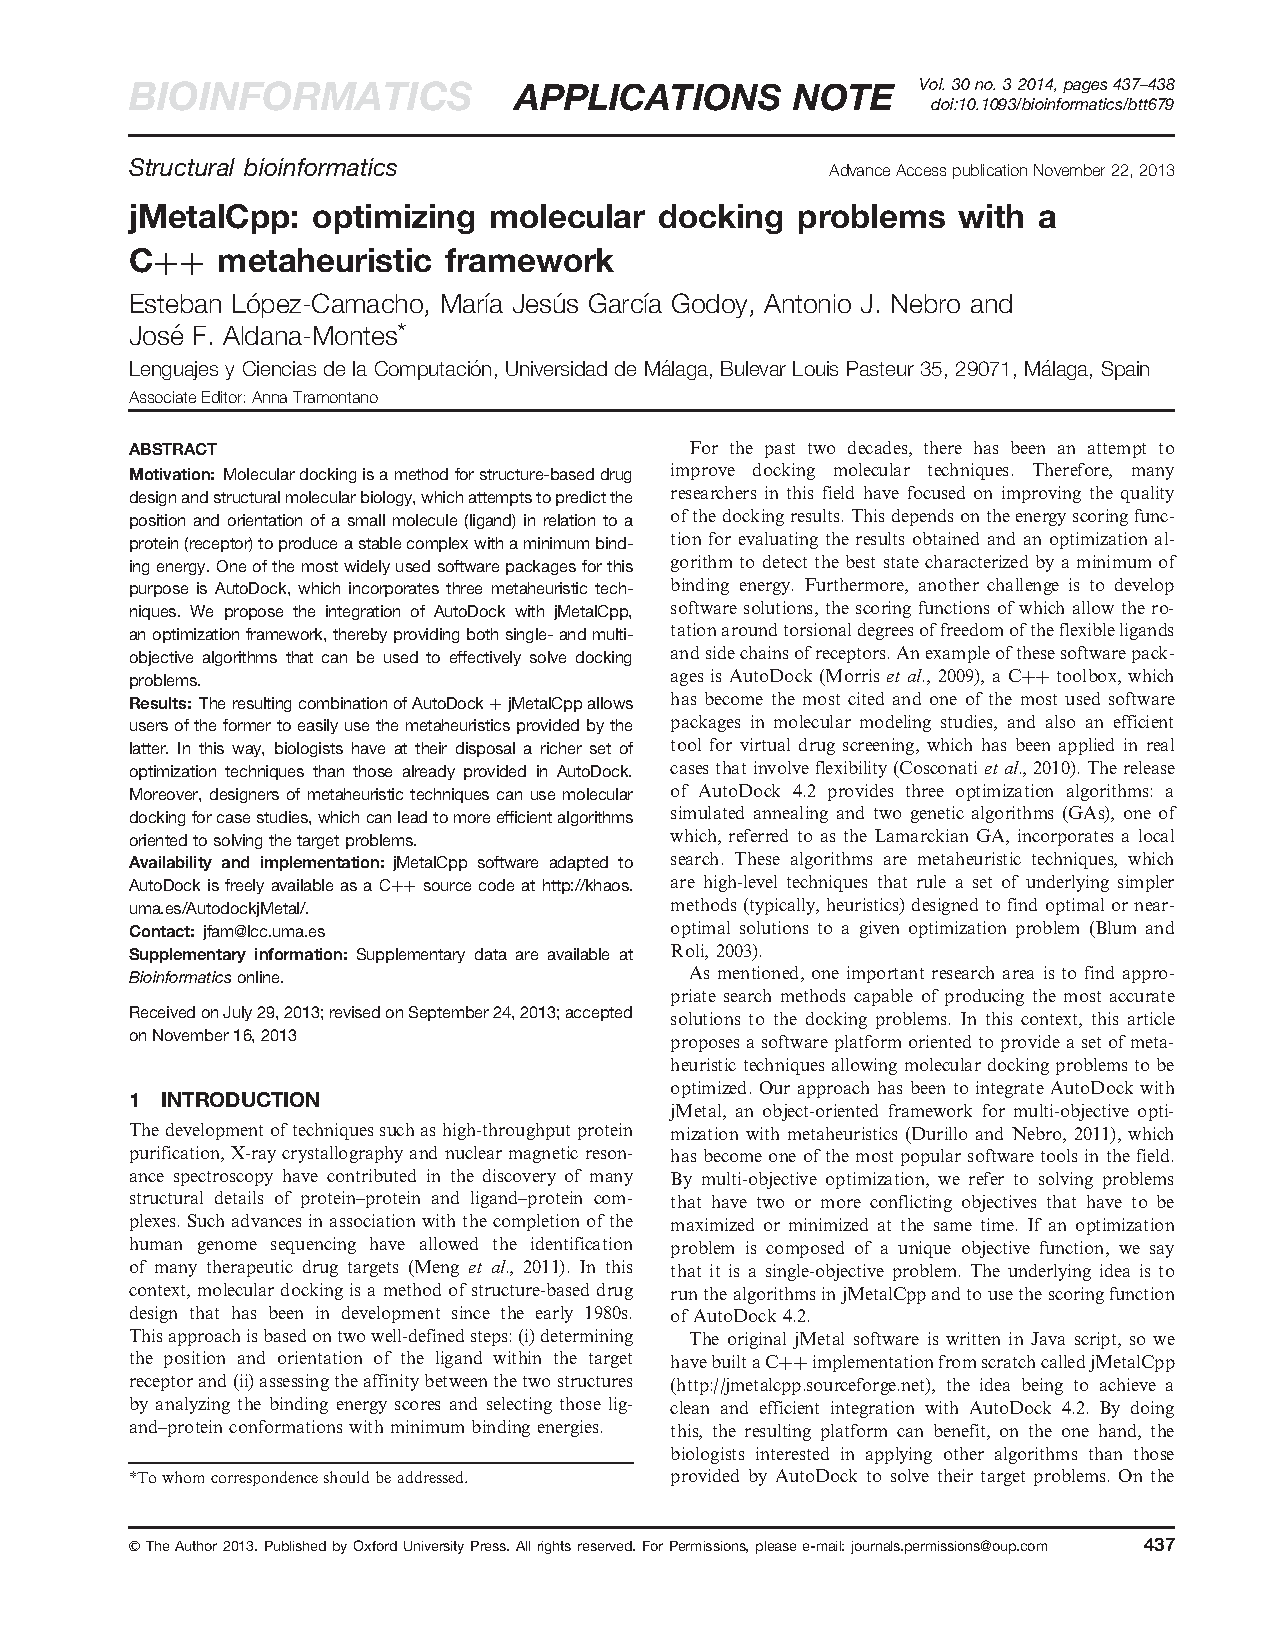
\includepdf[pages=-,scale=0.83,pagecommand={\pagestyle{fancy}}]{pdf/bioinformatics.pdf}

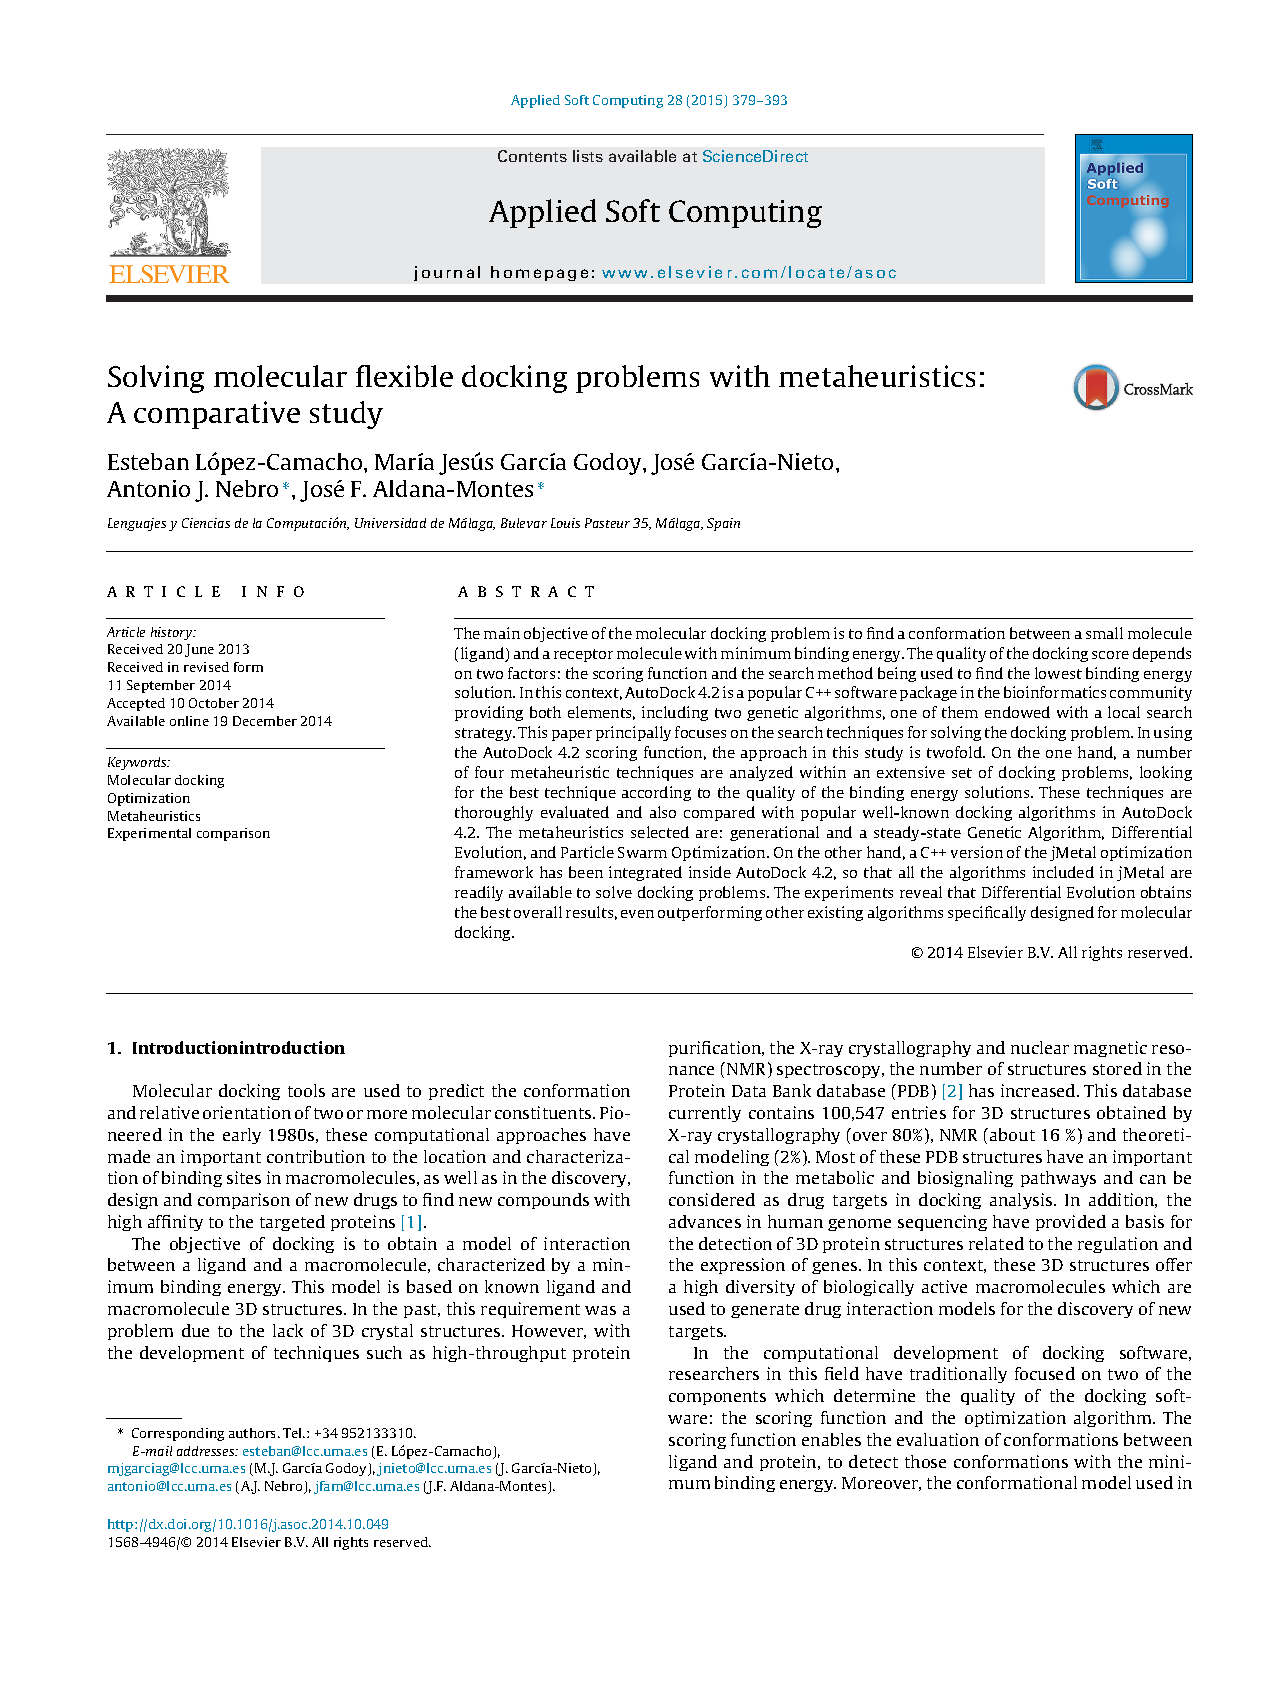
\includepdf[pages=-,scale=0.83,pagecommand={\pagestyle{fancy}}]{pdf/asoc.pdf}

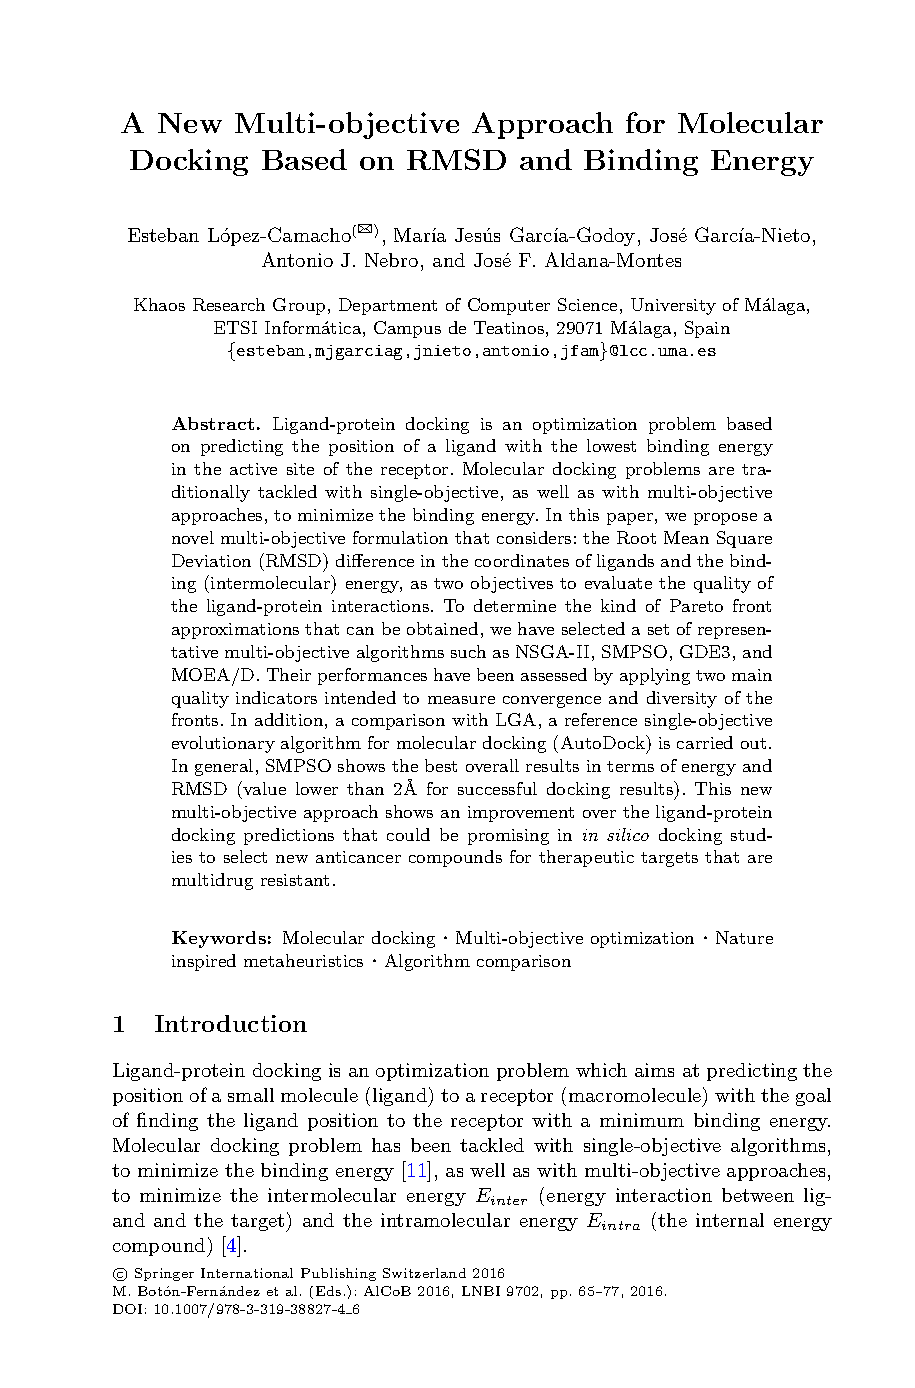
\includepdf[pages=-,scale=0.80,pagecommand={\pagestyle{fancy}}]{pdf/alcob.pdf}

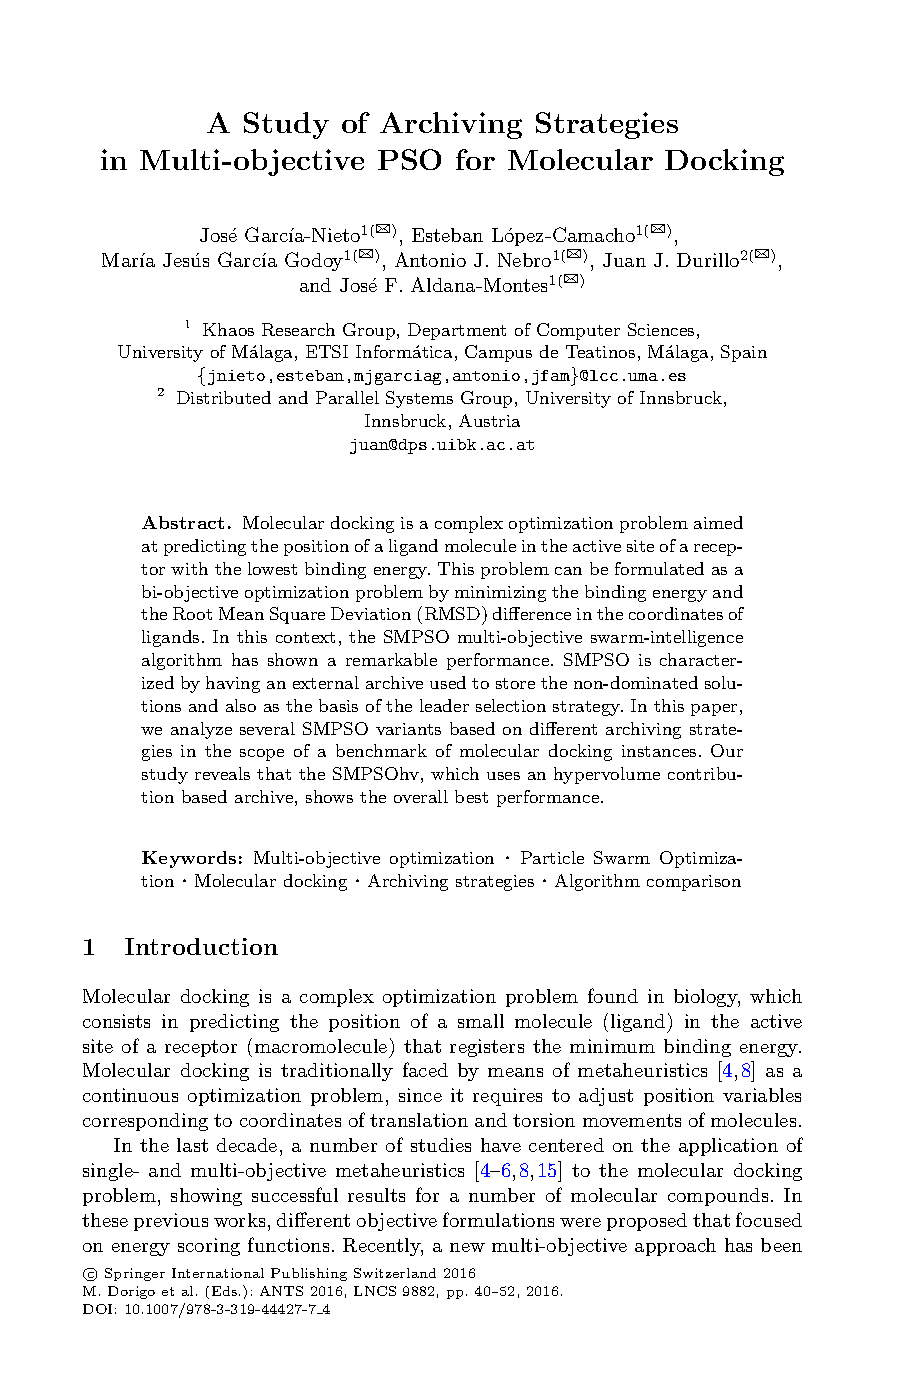
\includepdf[pages=-,scale=0.80,pagecommand={\pagestyle{fancy}}]{pdf/ants.pdf}
